\chapter{Grundlagen}

\section{Digitale Plattformen als disruptive Innovation}

\subsection{Definition und begriffliche Abgrenzung}

\newpage

\subsection{Wertschöpfung auf digitalen Plattformen}

\newpage

\subsection{Cloud-Computing auf digitalen Plattformen}

\newpage

\subsection{SAP Business Technology Platform}


\newpage


\section{Die deutsche Versicherungsbranche}

\subsection{Definition und Grundprinzipien der Versicherung}

Aufgrund der kontinuierlichen Weiterentwicklung des Versicherungsmarktes und der wachsenden Teilnahme unterschiedlicher Wirtschaftsdisziplinen an der Versicherungswissenschaft gibt es heutzutage eine Vielzahl von Definition für den Begriff der Versicherung. Wird sich bei dem Begriff auf die ökonomischen Gesichtspunkte konzentriert, wird in der Literatur insbesondere auf den Wirtschaftswissenschaftler Dieter Farny verwiesen, welcher das Versicherungsprodukt, auch Versicherung oder Police genannt, definiert als die: 

\glqq Deckung eines im Einzelnen ungewissen, insgesamt geschätzten Mittelbedarfs auf der Grundlage des Risikoausgleichs im Kollektiv und in der Zeit.\grqq \autocite[S. 8f.]{FARNY2011}

Folglich ist die Versicherung ein Produkt zur Deckung von Sicherheitsbedürfnissen, indem es Risiken auf eine Gefahrengemeinschaft, das Kollektiv überträgt. Die Befriedigung dieser Sicherheitsbedürfnisse umfassen die Absicherung von materiellen als auch beruflichen Risiken und sind auf der zweiten Ebene der Maslowschen Bedürfnispyramide zu finden. \autocite[Vgl.][S. 30]{BECKER2019} Das zugrunde liegende Konzept wird als Risikotransfer bezeichnet, bei dem der Versicherungsnehmer gegen Zahlung einer Prämie das Risiko auf den Versicherer überträgt. Beim Eintreten eines entsprechenden Schadens, dem Versicherungsfall, erhält der Versicherungsnehmer von der Versicherung einen Schadensausgleich. Dieser Risikoausgleichseffekt wird von Versicherungsunternehmen genutzt, um die systematische Übernahme von Risiken mit einem im Hinblick auf die Gewinnmöglichkeiten akzeptablen unternehmerischen Risiko durchzuführen. \autocite[Vgl.][S. 9]{FARNY2011}
Grundvoraussetzung ist hierbei, dass der Umfang der Schäden statistisch abschätzbar und dadurch der benötigte Beitrag jedes Mitglieds des Kollektivs mathematisch bestimmbar ist. Aufgrund dieser Kombinationen von Risikotransfer und Prämienzahlung werden Versicherungsunternehmen(VU) auch als Finanz- und Risikointermediäre bezeichnet. \autocite[Vgl.][S. 53]{ZWACK2017}

Grundsätzlich wird zwischen zwei Arten von Versicherungsunternehmen unterschieden: Erstversicherer und Rückversicherer. Erstere schließen ausschließlich Versicherungsgeschäfte mit gewerblichen Unternehmen, privaten und öffentlichen Haushalten ab, währenddessen Rückversicherer das daraus resultierende Risiko der Erstversicherer übernehmen.\autocite[Vgl.][S. 240f.]{FARNY2011} Im Rahmen dieser Arbeit werden insbesondere Kfz-Versicherer betrachtet, welche der Gruppe der Erstversicherer zuzuordnen sind.

Darüber hinaus sind deutsche Erstversicherer durch verschiedene regulatorische Anforderungen wie dem Versicherungsaufsichtsgesetz (VAG) und der Solvency II-Richtlinie der Europäischen Union verpflichtet, um die Stabilität und Integrität des Versicherungsmarktes zu wahren. \autocite[Vgl.][]{BAFIN2016} Eine der fundamentalen Vorschriften ist die Spartentrennung nach § 6 II VAG. Demnach müssen Erstversicherungsunternehmen getrennte Geschäftsbereiche für Lebens-, Kranken- und Kompositversicherungen führen. Zu Gruppe der Kompositversicherungen, welche auch als Schaden- und Unfallversicherung bezeichnet wird, zählen seit dem 30.06.1990 alle Versicherungen, die nicht zur Lebens- und Krankenversicherung gehören. \autocite[Vgl.][S. 241-243]{FARNY2011} In der Praxis führt das Spartentrennungsprinzip häufig zur Bildung von größeren Mutterkonzernen, bei denen eine Holding über mehrere rechtlich selbstständige Versicherungsunternehmen verfügt. (siehe Abbildung \vref{fig:StVKonzern}). Eine beispielhafte Konzernstruktur der AXA SE ist im Anhang ... zu entnehmen. \autocite[Vgl.][S. 241-243]{AXAKONZERNSTRUKTUR2023}

\begin{figure}[h]
    \centering
    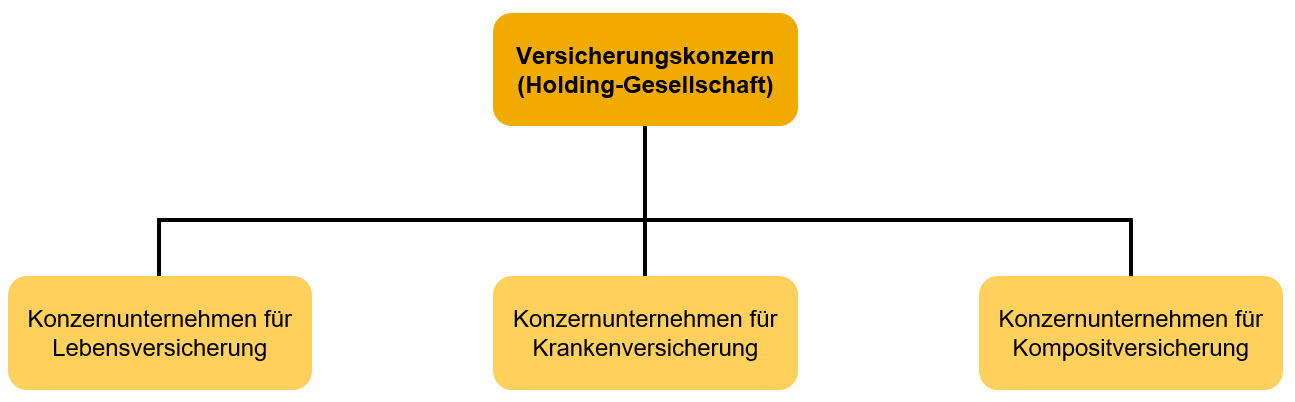
\includegraphics[width=1\textwidth]{img/Struktur_VKonzern2.jpg}
    \caption[Struktur eines Versicherungskonzerns]{Struktur eines Versicherungskonzerns\autocite{StVKonzern}}
    \label{fig:StVKonzern}
\end{figure}
\footnotetext{Vgl. eigene Darstellung angelehnt an: Nguyen, 2013, S.172}

\newpage

\subsection{Aufbau und Besonderheit der Kfz-Versicherungssparte}

\newpage
